
\section{Model of computation}

Consequently, people began to look at how to parallelize algorithms and compare them through computational models to determine which ones performed best. The notions of complexity have been adapted to this new context and we have seen the emergence of many algorithms often presenting very elegant solutions. In this section, we will give a quick review of different models of computation which exist to compute the complexity of algorithms on parallel systems. There are countless of them with as many variations, we will limit ourselves to a ``canonical'' subset, the most famous ones and that will lead us to a particular computation model.

% Cache oblivious ? http://repository.cmu.edu/cgi/viewcontent.cgi?article=1104&context=compsci

% Interesting
% https://pdfs.semanticscholar.org/1417/c585009393cc2b45a38939a5e818738c62ea.pdf
% http://citeseerx.ist.psu.edu/viewdoc/download?doi=10.1.1.958.9741&rep=rep1&type=pdf

\subsection{PRAM}

This model was introduced in 1978 by S. Fortune and J. Wyllie~\cite{fortune1978parallelism,wyllie1979complexity}. They knew that we could not keep increasing performances of computers forever and therefore that one solution to this problem was to introduce parallelism in the computations. But, at that time, not many tried to determine what was the theoretical power of such machines.

The parallel random access machine (PRAM) can really be seen as an extension of the classical RAM model~\cite{cook1972time}. It describes an unbounded set of processors, with an infinite global memory and a set of input registers. Each processor has its own accumular, unbounded local memory, program counter and a flag which indicates whether or not the processor is running; there are also a list basic of instructions (load, store, add, jump, read) and some specific (fork and halt). The idea was to remain relatively close to the programming languages of the time while presenting a certain abstraction necessary to calculate the complexity of the various algorithms.

Its main specifities are the fork instruction, which initializes an inactive processor to start at a label, and the halt to stop running, other instructions are assimilated to the assembler's expression capacities. Traditionally, several processors are allowed to read simultaneously the same data but only one can write at a time on a specific cell; this assumption is often supported by the majority of materials designed as MIMD and is one of the possibilities offered by the model which can propose exclusivity or concurrency as well on the readings as on the writings since each instruction is executed in a cycle of three phases: a read (if any), a computation and a write (if any).

But most importantly, it defines classes of complexity where execution is determined on termination of the first processor. Hence, the time to accept an input is the minimum over all the computations from the first processor. Therefore, deterministic and non deterministic $T(n)$-TIME-PRAM classes are classically defined, some equivalences were also proven: $T(n)$-TIME-PRAM = $T(n)$-SPACE or N-$cT(n)$-TIME-PRAM = N-$2^{cT(n)}$-TIME (for $T(n) \geqslant \log(n)$)~\cite{fortune1978parallelism}.

For the first theorem, one should observe that the number of machine configurations in $T(n)$ algorithm is bounded by $2^{dT(n)}$. Then the equivalence is described as follow, the first processor is able to launch $2^{dT(n)}$ processes in $O(T(n))$, each holding a different number representing one configuration. They all decode their given configuration, compute the next one and encode it. Finally, to determine if the word is accepted from the initial configuration, it is sufficient for each processor to search for the successor configuration of the successor iteratively until we reach the termination state from the initial one (path-doubling strategy); all these operations can be performed in $O(T(N))$.

For the second, a similar argument can be used, each processor can guess one symbol of computation. The first $n$ processors check initial tape configuration, the others check that the symbol they consider corresponds well to that of the transition from the previous configuration and neighboring symbols. The latest processors must also verify that the state is accepting.

Many theoretical results on the bounds of algorithms were also obtained on models with slight variations in comparison to the original one~\cite{karp1988survey}. However, this model has some characteristics that make it unrealistic in practice. Indeed, there is no limit on the number of processors available on the machine. All basic operations are in constant time while some are obviously slower than others. Each processor can access any data and from anywhere, there is no difference between shared and distributed memory. Resource access management is simply ignored, there are no data contentions for instance. But it has the advantage of offering a working environment close to the mental conception of the problem.

\subsection{BSP}

Bulk Synchronous Parallel (BSP) was introduced in the late eighties by L. Valiant~\cite{valiant1990bridging}. It was designed to lie inbetween hardware and programming models, in the same way that the von Neumann machine is comparable to the Turing machine. This computer consists of three parts: \textit{components} able to perform processing (asynchronously) and memory operations, a \textit{router} which dispatchs the messages between pairs and a primitive (like a barrier) which allows synchronisation of all or only a subset of processors. This aims to symbolize the three main steps involved in any parallel algorithm, concurrent computing, communication and synchronization. This model thus makes it possible to represent other aspects which intervene in this type of algorithm and does not concentrate only on the computational complexity of the problem.

A computation, in this model, is described as a sequence of \textit{supersteps}. Each superstep is divided into three stages, a first where each component is allocated a task consisting of some local computation, then a communication phase is realized in order to propagate the results thanks to message transmissions and (implicitly) message arrivals from other components. Finally, after each period of $L$ time units, a global check is made to determine whether the system managed to accomplish the work within the allotted time. If it has, the machine can proceed the next superstep. Otherwirse, a new period is allocated to terminate the current superstep. Those $L$ units of time are called \textit{periodicity} and can be controlled at runtime. The lower bounds are set by the material capacities while the upper ones are rather software, by design, and related to the granularity of the solution since to achieve the optimal processor utilization, in each superstep, each processor should be assigned a task of approximately $L$ steps.

Some constants are defined like the communication bandwidth, the size of the local memory, the number of local operations per period or the maximal number of messages per superstep; some considerations about timings and relative proportions are also established. Hence, the cost of an algorithm is defined as the sum of three terms, the cost of the longest running local computation, the cost of communication inbetween processes and the cost of the synchronisation barrier (latency) at the end of the superstep. Each of them being summed on the number of supersteps needed to solve the problem.

The model knew many variations on the same theme and was recently updated to include several layers of cache\index{Cache} and the notion of optimality without paying attention about the parameters, also known as \textit{oblivious}~\cite{valiant2011bridging}.

Note that the MapReduce model, introduced by Google in 2004~\cite{dean2008mapreduce}, is based on similar concepts and can be reduced to it~\cite{senger2016bsp}. It focuses mainly on problems related to Big Data and provides a more practical framework. The data is first loaded and distributed between the different processors. Each then applies a function \textit{map} that transforms the local data and writes the result into a temporary storage area. The results are then redistributed on the basis of keys, also produced during the map operation, so that all the data belonging to the same key are sent to the same processor, this is the big \textit{shuffle}. Finally, each processor reworks those new data by key in parallel, \textit{reduce}. There are thus two ``BSP supersteps'' in one in this model.

\begin{figure}[!ht]
\centering
\begin{minipage}{.5\textwidth}
  \centering
  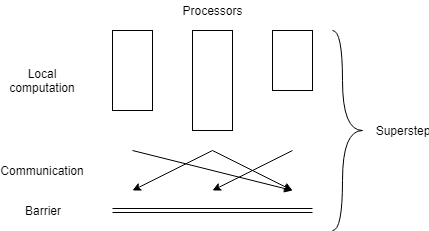
\includegraphics[width=0.9\linewidth]{Chapters/GPU/BSP.png}
  \captionof{figure}{BSP}
  \label{fig:BSP}
\end{minipage}%
\begin{minipage}{.5\textwidth}
  \centering
  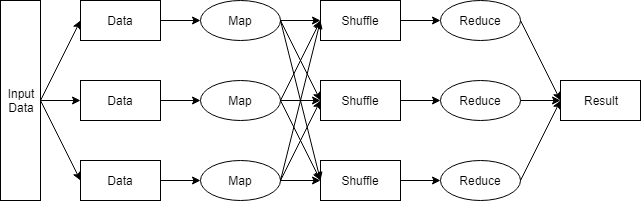
\includegraphics[width=0.9\linewidth]{Chapters/GPU/MapReduce.png}
  \captionof{figure}{MapReduce}
  \label{fig:MapReduce}
\end{minipage}
\end{figure}

\subsection{LogP}

The canonical PRAM model, even though it proposes nice theoretical results, is not representative of real-life computers due to its zero communication delay, synchronism among all the execution steps or infinite bandwidth. On the opposite, BSP may represent a too large variety of machines whereas we see a convergence towards a same architecture for distributed computing: many complete computers connected by a communication network. LogP model proposed in 1993 by Culler and al.~\cite{culler1993logp} tried to take place inbetween those two models. It focuses on high level abstraction of the machine and target essentially communication (message-passing style).

Some parameters are defined such as an upper bound on latency $L$ incurred by sending a message from a source to a destination, an overhead $o$ linked to the inactivity of the processor while sending or receiving messages, a gap $g$ defined as the minimum time between two consecutive messages and $P$ the number of processes. This model assumes that the network has a finite capacity ($\frac{L}{g}$ messages from any one processor to any other), asynchronous communication and messages are expected to be small, 

The BSP and LogP models focus on different concepts, they do not aim at the same purpose. For BSP, barrier synchronisation and routing of messages are primitives and is much likely used to design algorithm. Whereas LogP proposes a better control of resources with loose synchronisation. But, more importantly, they propose a comparable power of computation to design algorithms and so BSP tends to be easier to manage and provides a more convenient programming abstraction~\cite{bilardi1999bsp}.

\subsection{PDM}

Aggarwal and Vitter introduced in 1988~\cite{aggarwal1988input} the external memory model (EM) or disk access machine (DAM) which counts the number of block\index{Block} I/Os to and from an external source of memory. The idea was that, at the time, the memories were too small to hold the entire dataset, so it was necessary to regularly fetch the data from an external source (i.e. magnetic tapes). EM algorithms explicitly control data placement and transfer to reduce the number of data queries to be made and their inherent slowness, disk accesses are 1 million times slower than the execution of one instruction on modern computer.

Once the desired data location has been found on the tape, accessing neighboring data is very simple. And since we also tend to want to access information located nearby (as in the case of a for loop), it can be interesting to amortize the relatively long initial delay to access a data by transferring a large contiguous group of data items at a time. We use the term \textit{block}\index{Block} to refer to the amount of data transferred to or from one disk in a single I/O operation.

With an analoguous spirit, Vitter and Shriver introduced the parallel disk model (PDM) which combines the notion of locality of references and the parallel accesses. All the processors read in main memories and many blocks\index{Block} of data can be swapped from different disks in parallel. Those models really captured the essential notions to exploit the locality as well as the load balancing to deserve our programs. Many results were achieved through these models and Vitter compiled many algorithms, with their analysis and their associated data structure in one interesting book~\cite{vitter2008algorithms}. Interests about technical difficulties and their practical solutions are also suggested but the main interest relies on sequential algorithms.

PDM uses the following main parameters: $N$ the problem size, $M$ the internal memory\index{Cache} size, $B$ the block\index{Block} transfer size, $D$ the number of independent disk drives and $P$ the number of processors.

Such that, in a single I/O, each of the $D$ disks can simultaneously transfer a block\index{Block} of $B$ contiguous data items. The data needs to be placed in internal memory $M$\index{Cache} in order to be able to perform the appropriate processing. The parallelism proposed by this model must be considered more as a weaker form, since the memory is distributed, each processor has its own internal memory and attached set of disks. It could be seen more as $P$ copies of EM machines.

\subsection{PEM}

As the external memory model (and its brother ``cache-oblivious''\index{Cache oblivious}) brings the notion of cache\index{Cache} and memory transfers to the RAM model, PEM realizes the same idea but with PRAM model. Bender et al., tried in 2005~\cite{bender2005concurrent}, to combine the notion of cache-oblivious\index{Cache oblivious} with parallelism but were more focused on one specific data structure, a B-tree\index{B-tree}. The underlying idea was that the cache\index{Cache} can be viewed as a bounded memory which can read or write from an external and global memory.

Finally, L. Arge, M. T. Goodrich, M. Nelson and N. Sitchinava, in 2008~\cite{arge2008fundamental}, came up with Parallel External Memory (PEM) model. It can be viewed as a single-disk external memory shared by several processes all owning a private cache\index{Cache}.

This model differs fundamentally from the previous model of computation as it keeps some shared memory. There is only one external data source that can be accessed by any processor. Nonetheless, each processor has its own internal memory, which introduces thus problems related to concurrency and data consistency. Be aware that no mechanism of synchronisation or communication among processors are provided and further extensions exist to treat the concurrent reads and writes.

It also makes the assumption that the performances are bounded by the I/O and its intrinsic latency. This model is defined by few parameters, $N$ the problem size, $P$ the number of processors, $M$ the cache\index{Cache} size and $B$ the block\index{Block} size. So the parameters are essentially the same than the previous one, the only difference is that there is only one disk.

\begin{figure}[!htb]
    \centering
    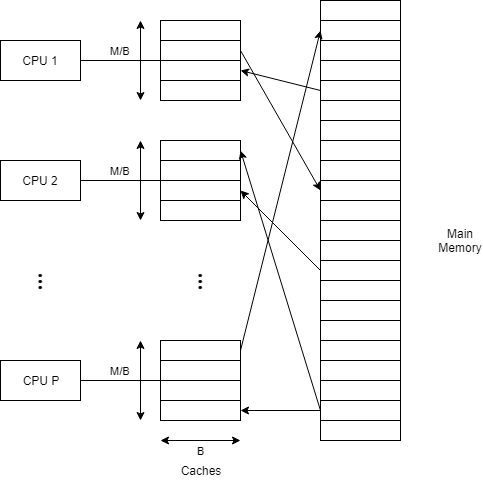
\includegraphics[width=0.5\linewidth]{Chapters/GPU/PEM.png} 
    \caption{PEM model}
\end{figure}

\subsection{TMM}

Threaded Many-core Memory model of computation was described in 2014 by L. Ma et al.~\cite{ma2014memory}, it wants to stay relatively close to the architecture found in GPUs. This model explicitly models the large number of threads per processor and the memory latency to slow memory. It mainly proposes finite constraints on the execution (on the contrary of the model PRAM which does not bound the number of processors) while not targeting a precise hardware or trying to calibrate the performance model.

It is defined by six parameters linked to I/O complexity: the time for a global memory access, the number of processors, the number of elements transfered per block\index{Block}, the size of the local memory\index{Cache} attached per group, the number of cores per group and the maximal number of threads per core.

As well as other parameters which are determined by the algorithm and more in relation to time complexity and PRAM notions. We find the total amount of work and per thread, the number of threads per core and the amount of memory space required per each thread. It is one of the many models which exist, but it offers both time and I/O complexity analysis. One can therefore expect stronger optimality criteria, if the algorithm is both optimal in time and in I/Os.

\subsection{Quantitative model}

More recently, people try to model the architecture of the GPU and their relative operations more accurately~\cite{baghsorkhi2010adaptive,hong2009analytical}. The idea was to find out bottlenecks in the implementation through static analysis and to provide tips for the developpers. Highlight operations that are supposed to be slow such that the user can be able to optimize them; or propose metrics to guide compiler optimization passes.

Hence, they go much more further in the concepts which intervene in the modelisation and provide more adhoc comparisons of implementations with the relative timing of each instruction. They represent the code through a work flow graph which feeds the computation and memory pipelines. Warps, SIMD instructions\index{SIMT} and other factors (like the number of threads, the block size, the cache size...) which may come into account while tuning performances are also taken into consideration. Considerations for which more explanation will be provided in the following section$^{[\ref{GPU}]}$.
